%\documentclass{beamer}
\documentclass[handout]{beamer}

\usepackage{pgfpages} 

%\setbeameroption{show only notes}

\usetheme{default}

\mode<presentation> {
%  \usetheme{Warsaw}
  \usetheme{Frankfurt}
%  \usetheme{Boadilla}
%  \usetheme{Marburg}
}

\mode<handout>{\setbeamercolor{background canvas}{bg=black!5} %
    \pgfpagesuselayout{4 on 1}[letterpaper,border shrink=4mm,landscape] %
    \setbeameroption{show notes}}

\title[CAC High Performance Math] {High Performance Math}
\author{Brock Palen\\ \texttt{brockp@umich.edu}}
\date{TBD}

\begin{document}
  \setbeamercovered{transparent}  
  \begin{frame}
    \titlepage
  \end{frame}

%table of contents
  \begin{frame}{Outline}
    \tableofcontents
  \end{frame}
 
\begin{frame}{References}
 \begin{block}{References}
  \begin{itemize}
   \item U.C. Berkeley CS267 Jim Demmel \\
     \url{http://www.cs.berkeley.edu/~demmel/cs267/}
   \item Numerical Algorithms Group     \\
     \url{http://www.nag.com/lapack-ex/}
   \item Basic Linear Algebra Subprograms \\
     \url{http://www.netlib.org/blas/}
   \item Linear ALgebra Package         \\
     \url{http://www.netlib.org/lapack/}
  \end{itemize}
 \end{block}
 \note{
   All Traning docs are available at \url{www.umich.edu/~brockp} \\
 } %end note
\end{frame} 



\section{Concepts}
\subsection{Terms}
\begin{frame}{Terms}
 \begin{block}{Terms}
  \begin{itemize}
   \item<1-> Bandwidth - Speed in GB/s of memory to CPU
   \item<2-> Floating Point Number - Floats and Doubles (1.2 5.002)
   \item<2-> Fixed Point Number - Ints (1 50 1,000)
   \item<3-> Floating Point Operation (Flop) - A mathematic operation on a floating point number
   \item<4-> Memory Refernce - A call to memory for data
   \item<5->  $q=f/m$ - Ratio of Flops to Refernces
   \item<6-> Cache - Fast memory local to the cpu
  \end{itemize}
 \end{block}
 \note{
  Most HPC applications require floating point calculations thus focus is on FLOPS and not fixed point performance. \\
  Data in cache is assumed to be latency free. It is also assumed to have enough bandwidth to feed the CPU.
 } %end note
\end{frame}
 \subsection {Memory vs CPU}
 \begin{frame}{CPU Speed}
  \begin{block}{CPU Perfromance}
   \begin{itemize}
    \item <1->Moore's Law
    \item <2->Focus and Rightly So
    \item <3->Multi-Core
    \item <4->Single Instruction Multiple Data (Vector)
   \end{itemize}
  \end{block}
  \note{
  \url{http://en.wikipedia.org/wiki/Moore's\_law} \\
  \url{http://en.wikipedia.org/wiki/SIMD}         \\
  \url{http://en.wikipedia.org/wiki/Vector\_processor} \\
  SIMD (SSE, 3DNow, AltiVec) is related to the vector CPU's systems like the NEC SX-9.  Vectors are for working on lists of numbers at the same time. It can be thought as a type of paralellism.  Most HPC Math Libraries make use of the SIMD unit on modern CPU's.  For example on the AMD Barcilona perfromance doubled in the SIMD (sse 128) unit. \\
  SIMD is very related to GP-GPU processing and CPU's like the IBM Cell. \\
 
  Cell CPU (PS3 and Road Runner)\\ 
  \url{http://en.wikipedia.org/wiki/Cell\_microprocessor} \\
  Computed Unified Device Arch. GP-GPU for Nvidia Cards
  \url{http://en.wikipedia.org/wiki/CUDA}
  } %end note
 \end{frame}

 \begin{frame}{Memory Speed}
  \begin{block}{Memory Performance}
   \begin{itemize}
    \item <1-> Memory Size
    \item <2-> Memory Speed (GB/s) trails CPU Flops
    \item <3-> Memory Latency is Worse than You think
   \end{itemize}
  \end{block}
 \end{frame}
 \note{
  Memory speeds matter more than latency. Modern CPUs like the AMD Opteron have the memory controler right in the cpu. This lowers memory latency.  It also adds total bandwidth (speed in GB/s) for an entire system in an SMP system. In such systems memory needs to be balanced across CPU Stockets.  
 } %end note
 \begin{frame}{Human vs. Computer}
   \[
    \alpha A=c
   \]
  \begin{block}{Sacle A Vector}
   \begin{itemize}
    \item<2-> 2n Flops
    \item<3-> 3n Refernces
    \item<4-> q=2/3
    \item<5-> \alert{Memory must be faster than the CPU}
   \end{itemize}
  \end{block}
 \end{frame}
 \note{
   While using sequences of simple operations like $AB=c$ and $ \alpha B=c$ are simple for a human to have organized it is a very slow type of operation for a computer. Computers need oprotunites for data reuse. \\
   BLAS 1 Functions: \\
   $AB=c$ is xDOT()  \\
   $\alpha B=c$ is xSCAL() \\
 These are the slowest of the BLAS operations.  Their ratio $ q=f/m $ is 2/3
 } %end note

\begin{frame}{Computers are Faster}
  \[ M[ \ddots ] A[\vdots] = B[\vdots]\]
 \begin{block}{xGEMV() Matrix Vector Multiplication}
  \begin{itemize}
   \item $ 2n^2 $ Flops
   \item $n^2+n $ Refernces
   \item $q=2$
  \end{itemize}
 \end{block}
 \note{
   These are the Blas 2 operations. They require that memory be half the speed of the CPU. We will see latter how in real world examples that because Blas 2 (and Blas 1) that there is not enough data reuse (none really) to allow the cache to keep the CPU fed.
 } % end note
\end{frame}

\begin{frame}{Computers are Faster Ctd.}
 \[ M[ \ddots ] N[ \ddots ] = C[ \ddots ] \]
 \begin{block}{xGEMM() Matrix Matrix Multiplication}
  \begin{itemize}
   \item $ 2n^3 \rightarrow n^3 $ Flops
   \item $ 4n^2 $ Refernces
   \item $ q=n/2 $
  \end{itemize}
 \end{block}
\end{frame}
 \note{
  Blas 3.  These calls are the basis of the LAPACK calls. Notice how as the size of M scales the ratio of flops (when coded right) increases to memory references.  The reason for this is clever coding can maximize reuse of data already requested from memory.  The vendor provided Blas libs will cleverly make sure that the data for an upcomming flop is already in cache. \\
User coded routines for xGEMM() are really a serious of xGEMV() calls. These operations cause data to be requested redundently from memory. \\
Users should always try to use Blas 3 calls even when they could be done with Blas 1 or 2.
 } % end note

\begin{frame}{Blas 1 \& 2 performance}
\begin{center}
  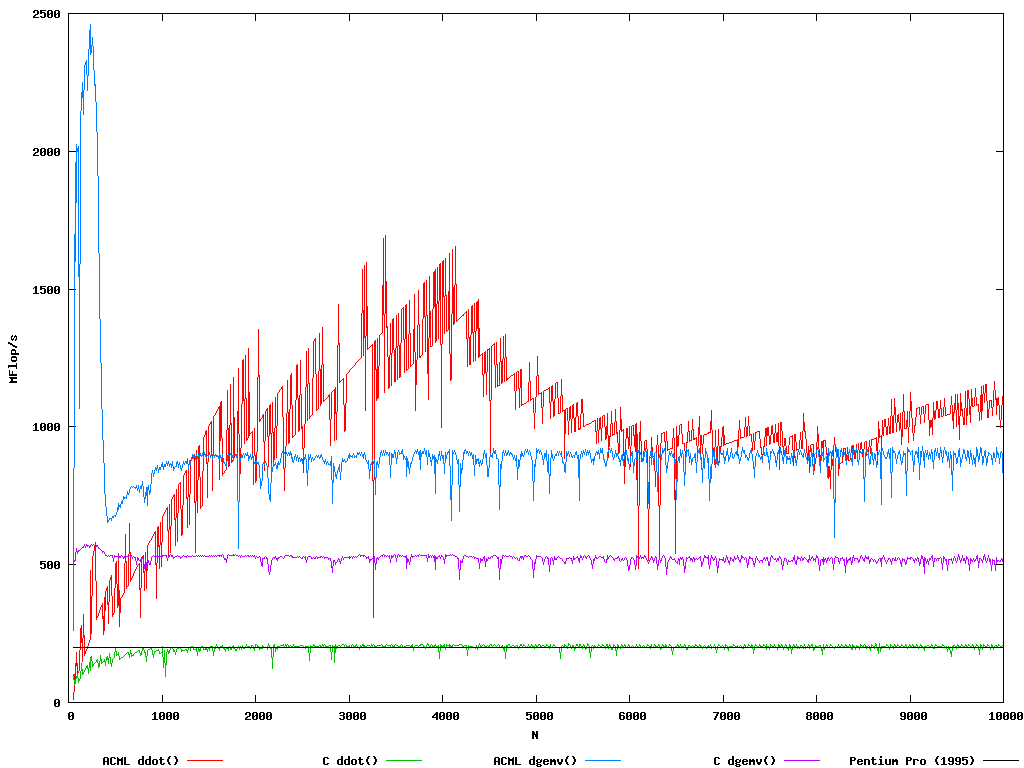
\includegraphics[height=3in]{blas12}
\end{center}
\note{
\begin{itemize}
 \item \texttt{pgcc -DACML -DBLAS1 -DBLAS2 -DBLAS3 blasSpeeds.c -lacml -pgf90libs -lpgftnrtl}
 \item \texttt{pgi/7.2 acml/4.1.0}
 \item opt2218  2.613 Ghz, 2flop/hz,  5.226 Gflop
 \item Pentium Pro 200 Mhz (1995) 1 FPU 200MFlop/s Peak
\end{itemize}
} % end note
\end{frame}

\begin{frame}{Blas 3}

\note{

} %
\end{frame}
\end{document}
